\documentclass{article}
\usepackage[utf8]{inputenc}
\usepackage[T1]{fontenc}
\usepackage{graphicx}
\usepackage{amsmath}
\usepackage{wrapfig}
\usepackage[top=1in, bottom=1.25in, left=1.1in, right=1.1in]{geometry}

\title{Reporte - Actividad 4: Introducción a la Programación de los Intérpretes de Comandos}
\author{García Monge Itzel Alexia}
\date{15 de Febrero, 2018}

\begin{document}
\maketitle
\section{Introducción}
En el siguiente reporte se habla sobre los usos básicos e introductorios de los comandos de UNIX, el cual es comúnmente conocido como Shell. Se realizaron ejercicios básicos que permitieron dominar los usos más indispensables, como lo es bajar archivos, filtrar y excluir palabras, mover información a un documento, cambiar permisos a ejecutables, observar el contenido de los archivos, incluso verificar si todos nuestros archivos estuvieran completos. Asimismo, se obtuvo una más breve pero igualmente necesaria introducción sobre distintos comandos en Emacs y para que sirven, como lo es vaciar la memoria, seleccionar, ir al principio o final de un documento, entre otros.

\section{Actividades a Realizar}
Empezamos la actividad creando una carpeta nueva dentro de Física Computacional I, la cual recibe el nombre de $Actividad4$. Con la carpeta creada, descargamos el script proporcionado de la página de pbworks llamado $script1.sh$ en la carpeta $Actividad4$ y lo abrimos en el editor de textos $Emacs (GIU)$. Adentro de la carpeta, abrimos la terminal y escribimos "echo \$SHELL" para empezar la actividad. 

El script que obtuvimos nos permite descargar los sondeos realizados por alguna estación, así que retomando de la actividad anterior buscamos el número de la estación utilizada, agregándola después de la variable $\textbf{STATION=}$, eliminando el  número de la estación que venía por default. Además, eliminamos todos los años que aparecen en el listado LISTYs= excepto por el año 2017 para obtener 12 archivos, uno para cada mes.  

    \begin{center}
    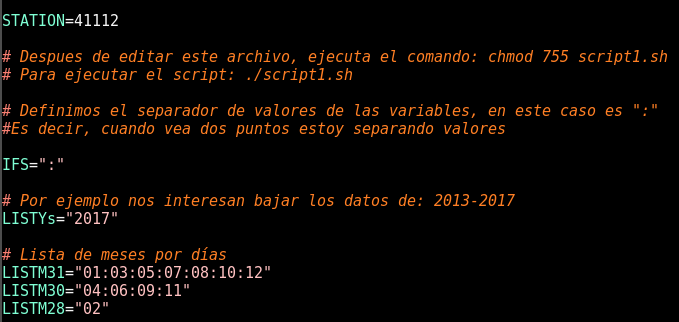
\includegraphics[height=5cm]{STATION.png}
    \end{center}

Con esto, nuestro script tiene las modificaciones necesarias para usarse, pero no para ejecutarse, es decir que si tratamos de ejecutar el script no podríamos. Esto ocurre ya no se tienen los permisos necesarios. Si vamos a la terminal y corremos el comando de $\textbf{ls -alg}$ se nos imprimirá en pantalla un listado de datos de la carpeta. Al inicio de cada archivo vienen una serie de guiones y letras, estas son los permisos.

	\begin{verbatim}
    -rw-r--r--
    -rwx-r-xr-x
    \end{verbatim}
    
Para entender qué están diciendo los permisos hay que retomar memoria de los bits, pero antes debemos separar qué es cada cosa, es decir, qué permiso está recibiendo quién. En primer lugar, el primer guión representa el archivo, mientras que los siguientes tres espacios son los permisos que tiene el dueño del archivo, los siguientes tres espacios son los permisos que tienen los demás usuarios que están conectados al archivo, y los últimos tres son los permisos para otras personas que deseen ver el archivo. Cada tres espacios tiene un valor, el primer espacio equivale a 1, el segundo al 2, y el tercero 4. Con el primero valor sólo puedes ver el archivo, con el segundo lo editas, y con el tercero lo ejecutas. Si nos fijamos en el permiso que tenemos, podemos observar que no tenemos activo el permiso para ejecutar, solo el de leer y modificar. 

Para cambiar nuestro permiso de $655$ debemos usar el comando $\textbf{chmod 755 script1.sh}$, logrando cambiar nuestro permiso a ejecutable. Corremos ahora el archivo, descargando desde la terminal los sondeos seleccionados y los colocandose en la carpeta $Actividad4$.
    
Si deseara observar todos los sondeos que se realizaron en el mes de enero una vez que la descarga haya finalizado, simplemente escribo en la terminal el comando $\textbf{less sounding*[tab]}$, creando que me imprima en pantalla todos los sondeos seguidos de enero en la terminal. El tab te pone automáticamente el nombre del primer archivo, en este caso enero. Si fueras a presionar tab dos veces, abrirías Febrero, tres veces te pone el nombre del archivo de Marzo y así sucesivamente. Esto es porque escribir asterísco después de sounding (*) hace que me seleccione todo lo que sigue de la palabra. Cuando hayamos observado todo lo que queríamos ver y necesitamos volver a la terminal, presionamos el boton $q$ para salir.

    \begin{center}
    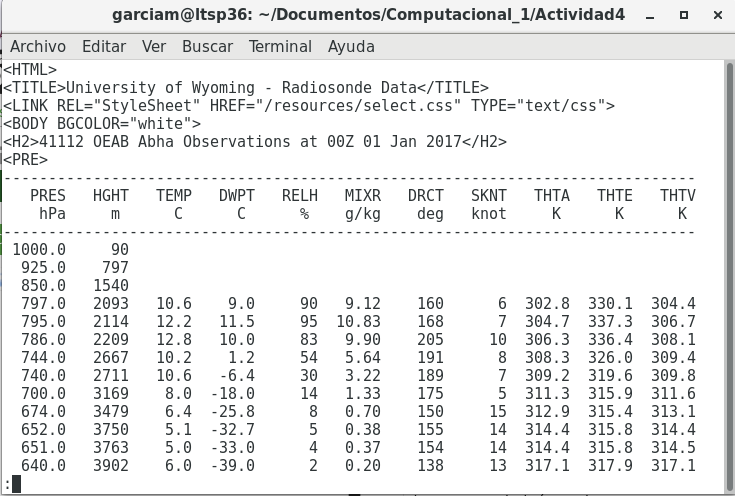
\includegraphics[height=7cm]{lessSound.png}
    \end{center}

Existe el comando $\textbf{cat}$, el cual nos imprime todos los sondeos en pantalla, pero a diferencia del comando anterior, pero este permite relacionar los datos la mostrar la información del archivo.

Al ser muchos datos los que tenemos, si queremos buscar algo de ellos en específico, tomaría mucho tiempo hacerlo manualmente, así que usamos en comando $\textbf{grep}$ y filtramos las palabras que nos interesan, imprimiendose en pantalla. Aún así, la mayoría del tiempo incluso lo que filtramos es demasiado, y queremos saber la cantidad de datos que logramos obtener sin perder tiempo contando. Para eso usamos el comando \textbf{wordcount} después de un pipe, apareciendo el número de renglones con esa palabra, número de palabras de todo lo obtenido, y el número de caracteres. El pipe (|) sirve para hacer cosas en serie, es decir, se hace una orden, se cumple, y se pasa a la siguiente con lo que se obtuvo para que haga algo nuevo con esa.

	\begin{verbatim}
	grep CAPE sounding*[presiona tab] |wc
    \end{verbatim}
    
Para saber con qué tipo de archivos estamos tratando, usamos el comando $\textbf{file}$ seguido del nombre, o inicio del nombre, de los archivos que queremos saber. En el siguiente caso podemos apreciar cómo se utilizó el comando en los archivos de texto descargado por el $script1.sh$.

    \begin{center}
    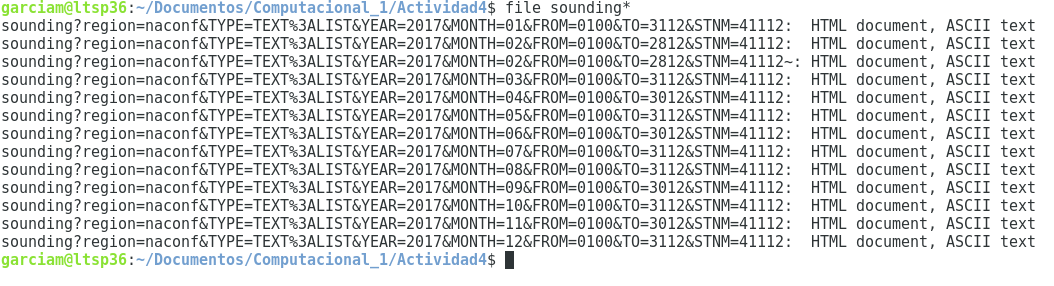
\includegraphics[height=5cm]{ascii.png}
    \end{center}

Mientras que imprimir en pantalla los valores que queremos obtener no está mal, la mayoría de tiempo se desean guardar esos datos en un documento que no se borre al cerrar la terminar. Para estos casos se utiliza el redireccionador $\textbf{>}$, el cual mueve los datos que desees a un archivo que tú mismo nombras al momento de ejecutar la acción. Por ejemplo:

	\begin{verbatim}
	cat sounding* > sondeos.txt
	\end{verbatim}
Crea el documento $sondeos.txt$, donde se guardaron todos los archivos con la palabra $sounding$ que se encontraban en la carpeta.

Pero así como queremos conseguir cierta información específica, hay veces que queremos excluir cierta información. Para excluir información se usa el comando $\textbf{egrep}$. Para nuestro caso, se quiso excluir toda la tabla de datos inicial y conservar solo lo que aparecía después, pero en un documento, por lo que se escribió:

		\begin{verbatim}
        egrep -v 'PRES|hPa' sondeos.txt | egrep '41112|Showalter|LIFT|
        SWEAT|K|Totals|CAPE|CINS|LFCT|CAPV|Temp|Pres|thick|Precip' > df2017.csv
		\end{verbatim}

Se puede crear un script en donde al ejecutarlo se puedan hacer las mismas acciones que escribimos en la terminal, como lo fue para crear el documento $sondeos.txt$ o $df2017.csv$ sin necesidad de escribirlo nuevamente. Se crea un script nuevo con esos comandos, cambiando el nombre del documento por $df2017_2.cvs$ y se ejecuta. Para comprobar que de verdad no hay diferencia con el script creado a mano en la terminal, se usa el comando $\textbf{diff}$ seguido de el nombre de los dos archivos que queremos comparar separado por espacios. Al presionar enter se observa que no ocurre nada, es decir, no se detecta ninguna diferencia entre el contenido de los documentos, pues efectivamente, contienen lo mismo.

    \begin{center}
    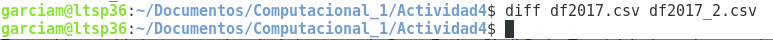
\includegraphics[height=0.9cm]{diff.png}
    \end{center}

\section{Síntesis Shell Script Tutorial}
\subsection{Introducción y Filosofía}
La programación con Shell ha adquirido algo de mala fama entre los administradores de sistemas. Esto ocurre mayormente por dos razones en específico. La primera siendo la velocidad en la que un programa interpretado correrá a comparación de, por ejemplo, un programa en C. El segundo problema aparece al escribir el código, ya que es muy sencillo escribir scripts de shell existen muchos de mala calidad.

Hay una gran cantidad de factores que pueden contribuir a un script de buena calidad, rápido y limpio. El criterio más importante sería el evitar comandos innecesarios sin importar el tamaño o propósito del script, al ser común que un script simple evolucione a uno más largo y complejo.

\subsection{Un Primer Script}
La primera línea del archivo empieza con un $\#!$, esto es un directivo especial que Unix trata de manera particular. El gato seguido del signo de exclamación indica que incluso si usas csh, ksh, o cualquier otro shell interactivo lo que siga deberá ser interpretado por el Shell de Bourne. Lo siguiente en la línea le dice a Unix que el archivo debe ejecutrarse por $/bin/sh$, el cual es una locación estándar del shell de Bourne en todo sistema Unix.

La segunda línea comienza con el símbolo $\#$, cuando este símbolo se encuentra solo—es decir, sin el signo de exclamación—marca la línea como un comentario y es ignorado completamente por el shell. En la tercera línea estamos llamando al programa shell con dos argumentos, $Hello$ y $World$, y no le interesa el espacio que haya entre ellos, automáticamente pondrá un espacio entre los parámetros. Pero si ahora agregamos comillas entre los argumentos, creando $"Hello    World"$, y lo corremos veremos que echo ha sido llamado con un solo argumento, así que lo imprimirá exactamente como aparece, incluyendo los espacios. Esto es por que el shell analiza el argumento antes de pasarlo al programa que llama, en este caso quita las comillas pero pasa el resto como un argumento.

Para correr el programa se escarbe $chmod 755 first.sh$, para hacer el archivo ejecutable y correrlo se usa $./first.sh$.

\subsection{Varables: Parte 1}
Casi todos los lenguajes de programación que existen tienen el concepto de variables, el cuál es un pedazo de memoria en el cual podemos asignar valores, leer y manipular el contenido, siempre van seguidas del singo $=$ o de lo contrario el script leerá la variable como un comando y tratará de ejecutarlo.

Si queremos guardar más de un valor en la variable debemos de escribir todo entre comillas para que el shell pueda utilizarlo como uno. Si la nombramos usando el comando $read$, se lee una línea desde la entrada estándar dentro de la variable suministrada y automáticamente pone comillas alrededor de su entrada, tratando a los espacios de la manera correcta. Puedes usar la variable del tipo que desees--real, entera--sin necesidad de declararla, pero si tratas de leer una variable sin declarar, el resultado es un espacio vacío sin advertencias ni errores, causantes de pequeños bugs.

Digamos ahora que quiere nombrar una variable y guardar su valor en un archivo. Normalmente un pensaría en nombrar una variable y después usar el comando de file, pero esto no funcionaría ya que el shell no comprende por si solo cuando se deja de nombrar una variable y empieza un comando. Para lograrlo se debe encerrar a la variable en llaves para que el shell sepa que esa es la variable y queremos aplicarle el comando que tiene al lado.

\subsection{Wildcards}
No es tan obvio saber que tan útiles son las wildwards en los scripts de shell, así que se proporcionarán  unos ejemplos. Primero, pensemos cómo se copiarían todos los archivos desde \textbf{/tmp/a} a \textbf{/tmp/b}, una opción es hacer:

\begin{verbatim}
$ cp /tmp/a/* /tmp/b/
$ cp /tmp/a/*.txt /tmp/b/
$ cp /tmp/a/*.html /tmp/b/
\end{verbatim}

Ahora, para ver la lista de los archivos en $\textbf{/tmp/a/} sin usar $\textbf{ls /tmp/a/} y cambiar su entensión de $*.txt$ a $*.bak$:

\begin{verbatim}
$ echo *.txt *.bak
\end{verbatim}

\subsection{Escape Characters}
La mayoría de los caracteres pueden evitar ser interpretdos al poner comillas entre ellos, así son tomados como son y se pasan al comando llamado. Sin embargo, existen algunos caracteres especiales, como \begin{verbatim}",$,'\\end{verbatim}que son interpretados por el shell aún cuando se encuentran entre comillas. Para lograr hacer que los caracteres no sean interpretados por el shell y pasen al comando siendo ejecutado usamos la barra invertida.

\subsection{Loops}
Casi todos los lenguajes tienen el concepto del $loop$ o bucle. Si queremos repetir una tarea veinte veces, no lo haremos escrbiendo el código veinte veces con ligeros cambios de vez en cuando. Como resultado a solucionar este problema tenemos $for$ y $while$ loops en el shell de Bourne.

Los loops $for$ iteran mediante un conjunto de valores hasta que la lista es terminada, mientras que los loops $while$ ingresan una variable antes de iniciar el bucle en un $\textbf{inut string}$ y tendrán corriendo al echo y los comandos de manera indefinida hasta que no se escriba la variable declarada. En algunos casos se declaran los dos puntos (:) en lugar de una variable para salir del bucle. Habrá veces en los que este método es necesario, pero es generalmente preferido usar una condición real para salir.
\begin{verbatim}
while [ "$INPUT_STRING" != "bye" ]
while :
\end{verbatim}

Otro truco útil es el bucle $while read f$, el cual trabaja con cualquier *nix y no depende de una línea de programa externa y usa el comando $case$ del cual se hablará más adelante. Lee desde el archivo $myfile$, y por cada línea proporciona el lenguaje que se cree está siendo usado. Cada línea debe terminar con un una línea en blanco, si un $cat myfile$ no termina así, esa última línea no podrá ser procesada. 

\subsection{Test}
$Test$ es una utilidad de comparación muy simple pero poderosa; puede usarse virtualmente para cada script de shell escrito aunque que no lo parezca al no ser llamados de manera directa. Los $test$ son frecuentemente llamados [, los cuales son sirven como un enlace simbólico para hacer los programas en shell más fáciles de leer. Es normalmente un built in, lo que significa que el shell mismo lo interpretará como $test$, incluso si el entrono es distinto. En otras palabras, [ es en realidad un programa como $ls$, así que debe de estar rodeado de espacios alrededor de todos los operadores.

Los $test$ son invocados de manera indirecta casi todo el tiempo via la declaración de $if$ y $while$. También es la razón por la que al crear un programa llamado $test$ habrá dificultades al correrlo, pues se llamará al shell builtin en lugar del programa recién creado.

\subsubsection{If...then...else...}
Los $if$ tiene la siguiente estructura básica:
\begin{verbatim}
if [ ... ]
then
  # if-code
else
  # else-code
fi
\end{verbatim}
Donde los comandos $if [...]$ y $then$ siempre deben de estar en diferentes líneas, o separas por un punto y coma, el cual suele usarse en condicionales simples. Nótese que $fi$ es $if$ al revés y se usa para terminal la condición.

Si se tiene más de una condición se agrega el comando $elif$ las veces necesarias, creando desde tres hasta los condicionales necesarios para correr el archivo. La barra inversa funciona de una manera opuesta al punto y coma: le anuncia al shell que no es el final de la línea y que la siguiente debe ser tratada como continuación de la actual. Esto es muy útil para un seguimiento fácil de lectura.

Existe una forma mucho más sencilla en la que podemos escribir los condicionales. En lugar de escribir $if$ y $else$ se usan los comandos $\&\&$ y ||, estos comandos dan código para correr si el resultado es verdadero o falso, respectivamente, siendo esta sintaxis posible al existir el built in de shell ]. Es recomendable tener cuidado con esta construcción ya que el usarlo de sobremanera puede llevar a la creación de códigos muy difíciles de leer, mientras que el uso de $if...then..else...$ crea una estructura mucho más entendible al lector. 

\subsection{Case}
Los casos, comúnmente llamados por su nombre en inglés $case$, salvan al programador de una gran cantidad de condicionales conservado una sintaxis sencilla. La línea de $case$ en sí es siempre del mismo formato, lo que significa que estamos evaluando el valor de la variable \textbf{INPUT STRING}.

Las opciones que entendemos son seguidas de paréntesis derecho, como $hello)$ y $bye)$. Esto indica que si la variable coincide con $hello$ entonces esa sección del código será ejecutada, si la variable coincide con $bye$ entonces otra sección del código será ejecutada. Existe un tercer paréntesis, el cual se escribe $*)$ que siempre debe de añadirse, ya que es la condición default que corre cuando ninguna de las opciones presentadas son ingresadas al momento de correr el archivo. 

Si desearamos salir completamente del script se tendría que usar el comando $exit$. Para terminar el caso se escribe $esac$, el cual es el reverso de la palabra $case$, para terminar los bucles escribimos $done$.

\subsection{Variables: Parte 2}
Hay un conjunto de variables ya establecidas que pueden utilizarse, pero a la mayoría no se le puede asignar valores. Estas variables contienen información útil la cual puede ser utilizada por el script para saber sombre el ambiente en el que está corriendo.

Algunas variables son:
\begin{itemize}
\item \$0				nombre base del programa de la forma en que fue llamado
\item \$1 ... \$9		los primeros 9 parámetros adicionales con el que el script fue llamado
\item \$@ 			todos los parámetros empezando desde el \$1, se recomienda utilizar
\item \$* 			similar a \$@ pero no preserva espacios en blanco, se recomienda evadir
\item \# 				número de parámetros el script fue llamado con, establecido automáticamente por shell
\item $shift$			permite tomar más de 9 parámetros
\item \$?				contiene el valor $exit$ del último comando que se corrió
\item \$\$ 			IDentificador de Proceso (PID en inglés) del shell
\item \!				PID del último proceso de fondo ejecutado
\item $IFS$			Separador Interno de Campo (IFS en inglés)
\end{itemize}

\subsection{Variables: Parte 3}
Las llaves, además de ayudar a crear separación entre variables y comandos, pueden lidiar con problemas de variables no identificadas o nulas. Si agreamos \textbf{:-} con las llaves puedes especificar algún valor default que quieras usar si la variable no está establecida.

Pasar el comando \textbf{-en} a $echo$ le avisa que no añada un salto de línea, aunque en algunos shells se usa \\c al final de la línea. La sintaxis \textbf{:=} establece la variable a su valor default si no está definida, esta técnica hace la variable siempre tenga algún valor en ella.

\subsection{Programas Externos}
Los programas externos son usados frecuentemente en scripts de shell, ya sea con comandos built in o comandos de utilidad Unix como $tr, grep, expr$ y $cut$. La apostrofe es el símbolo mayormente ascociado con comando externos, indica que el texto encerrado será ejecutado como un comando; simplemente obtiene la salida estándar de cualquier comando o conjunto de comando que elijamos correr. Además, mejora el rendimiento al querer correr un comando o conjunto de comandos lentos.

\subsection{Funciones}
Se pueden usar fácilmente funciones en los scripts generalmente de dos maneras: la primera es con un script simple en donde la función está declarada en el mismo archivo, la segunda--y más utilizada--es escribir una "biblioteca" de funciones útiles y citar ese archivo al inicio del script que desees. Las funciones no pueden cambiar los valores con el que fueron llamados, esto solo puede hacerse cambiando el valor de las variables mismas, no los parámetros pasados al script.

Una función puede regresar un valor de cuatro maneras distintas:
\begin{itemize}
\item Cambiar el estado de una o más variables
\item Usar el comando $exit$ para terminar el script de shell
\item Usar el comando $return$ para terminar la función y regresar el valor suministrado a la sección llamada del script de shell
\item $echo output$ a $stdout$ hara que sea atrapado por el $caller$
\end{itemize}

\subsection{Pistas y Tips}
Unix está lleno de utilidades para la manipulación de texto, haciendo que virtualmente todo bajo Unix sea texto. Virtualmente todo lo que se pueda pensar está controlado ya sea por archivo de texto o un comando de interface de línea (CLI).

Tomemos como ejemplo a $\textbf{tr}$, el cual es usado por su rango al poder convertir texto en subíndice o superíndice. Otras herramientas poderosas son $\textbf{awk}$ y $\textbf{sed}$. $\textbf{awk}$ funciona de manera similar a $scanf$ en C al quitar espacio en blanco no deseado, mientras que $\textbf{sed}$ elimina palabras del script, a diferencia de \textbf{tr} que elimina caracteres y \textbf{grep} que elimina líneas enteras.

\subsection{Referencias Rápidas}
Esta sección esta una rápida guía de referencia para los comandos menos fáciles de adivinar y códigs de script de shell. Por su naturaleza, son difíciles de encontrar usando motores de búsqueda. Estos ejemplos incluyes manejo de proceso, argumentos de scripts de shell y condiciones de evaluación de script de shell.

	\begin{center}
    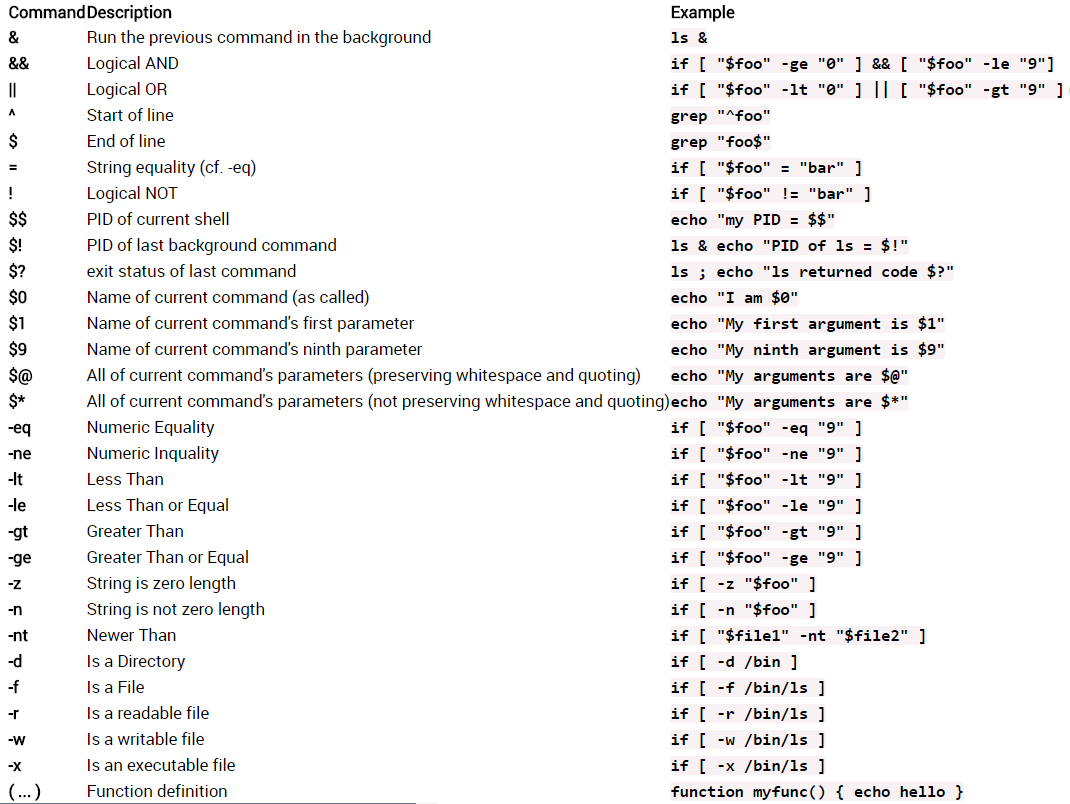
\includegraphics[height=10cm]{comandos.png}
    \end{center}
    
\subsection{Shell Interactivo}
Bash tiene herramientas de búsqueda muy prácticas. Las teclas $arriba$ y $abajo$ deslizan a través del historial de comandos previos, $ctrl=r$ hará una búsqueda en reversa juntando cualquier parte que se parezca a la línea de comando, $esc$ y el comando seleccionado será pegado en el shell actual para editarlo.

Ksh puede ser utilizado con más frecuencia añadiendo comandos del historial, ya sea en modo $in$, $vi$ o $emacs$. Hay un gran número de formas de la cual puede hacerse dependiendo de las circunstancias.

\section{Bibliografía}
\begin{itemize}
\item Detexify. Retrieved February 24,

$2018 http://detexify.kirelabs.org/classify.html$

\item Shell Scripting Tutorial. (n.d.). Retrieved February 24, 2018,

$https://www.shellscript.sh/index.html$

\end{itemize}

\section{Apéndice}
\begin{enumerate}
\item \textbf{¿Qué fue lo que más te llamó la atención en esta actividad?} Los nuevos comandos que se pueden realizar en la terminal usando UNIX. En general me gustaron mucho todos los nuevos comandos, como el descargar desde la terminar, el poder cambiar permisos, incluso el lograr filtrar ciertas parte del script a un nuevo archivo.

\item \textbf{¿Qué consideras que aprendiste?} Aprendí lo básico de una nueva forma de programar, o al menos una nueva forma de manejar datos desde la terminal, el cual tiene demasiadas ventajas y facilita el manejo de una gran cantidad de datos.

\item \textbf{¿Cuáles fueron las cosas que más se te dificultaron?} El comprender la diferencia entre el comando $less$ y $cat$, así como el manejo de los comando en Emacs, ya que me tomo tiempo darme cuenta que no funciona con los mismos comandos usados normalmente.

\item \textbf{¿Cómo se podría mejorar en esta actividad?} No le veo ninguna falta de algo, todo fue bien explicado y la ayuda fue proporcionada cuando fue necesaria.

\item\textbf{¿En general, cómo te sentiste al realizar en esta actividad?} Muy feliz, me gustó mucho aprender estos nuevos comandos y formas de realizar las cosas, fue muy divertido manipular tantos archivos y sentirlo todo tan fácil de recordar y seguir el hilo. No fueron comandos y formas de programar tan confusas como las actividades anteriores.
\end{enumerate}


\end{document}
